\documentclass[11pt]{article}
\usepackage[a4paper,margin=2.3cm]{geometry}
\usepackage[T1]{fontenc}
\usepackage[utf8]{inputenc}
\usepackage{lmodern}
\usepackage{microtype}
\usepackage{amsmath,amssymb}
\usepackage{graphicx}
\usepackage{booktabs}
\usepackage{tabularx}
\usepackage{multirow}
\usepackage[font=small,labelfont=bf]{caption}
\usepackage[numbers,sort&compress]{natbib}
\usepackage[colorlinks=true,linkcolor=blue!50!black,citecolor=blue!50!black,urlcolor=blue!50!black]{hyperref}

\newcommand{\pct}{\,\%}

\title{Borrowing from other patients, not from healthy brains: a pre-registered evaluation of calibration transfer for motor-imagery brain--computer interfaces after stroke}
\author{Author names and affiliations to be added}
\date{Draft, \today}

\begin{document}
\maketitle

\begin{abstract}
\noindent\textbf{Objective.} Motor-imagery brain--computer interfaces (BCIs) for stroke rehabilitation must be calibrated on each patient, and the few trials a patient can give leave decoders unreliable. Borrowing data from healthy participants is the usual remedy. We tested which source of borrowed data shortens calibration after stroke: healthy recordings, a physiology-based simulation of stroke EEG, an EEG foundation model, or other patients' recordings.
\textbf{Approach.} We harmonised two public stroke cohorts, 50 acute patients imagining left- versus right-hand movement and 24 chronic patients imagining moving the affected hand versus resting, together with 109 healthy participants. Each cohort kept a locked test set of patients never used during method development. Hypotheses were pre-registered in a version-controlled log, and every confirmatory analysis was run once. Per-patient Riemannian decoders were compared with deep transfer (EEGNet), a frozen foundation model (CBraMod), LesionSim (a simulator that edits healthy EEG to mimic weaker, shifted and more variable lesioned-side activity, including automatically learned settings), and pooling other patients' data into a re-centred Riemannian decoder.
\textbf{Main results.} With five calibration pairs, pooling other patients' data raised accuracy on the locked test patients from 77.1\pct{} to 81.4\pct{} (one-sided $p = 0.035$), the level the patient's own decoder reached only with ten pairs. Healthy data did not help in any form: deep transfer trailed the per-patient decoder by 4.5--12 points, the foundation-model probe by 14--24 points, and LesionSim closed none of the gap between healthy and real-patient donors. A calibration-only safety gate cut the number of patients harmed by transfer from 9 to 2 of 16. Left- versus right-hand imagery in acute stroke stayed near chance for most patients; a window ensemble gained 3.6--4.1 points without reaching significance on the locked test.
\textbf{Significance.} For few-trial stroke BCIs, pooling real patients beats simulating them. Code to rebuild the benchmark, a real-time implementation and the full pre-registration trail are released.
\end{abstract}

\section{Introduction}

Brain--computer interfaces that turn movement-related brain activity into feedback can improve upper-limb recovery after stroke. A meta-analysis of nine randomised controlled trials with 235 patients found a standardised mean difference of 0.79 in upper-limb Fugl-Meyer scores in favour of BCI-based therapy \citep{cervera2018}. Controlled studies that coupled sensorimotor desynchronisation to hand and arm orthoses \citep{ramosmurguialday2013} or to functional electrical stimulation \citep{biasiucci2018} reported clinically meaningful gains, lasting 6--12 months in the latter. Such therapy depends on a decoder that reliably detects the patient's attempt to move. Motor-imagery decoders are trained per user, and even healthy users vary widely: across 54 participants the mean accuracy was 71.1\pct{}, and 53.7\pct{} were classed as unable to use motor imagery proficiently \citep{lee2019}. Stroke patients can reach similar levels when a decoder is trained on their own data \citep{ang2011}. However, each calibration trial costs effort that patients early after stroke can rarely give, and the information the decoder needs may sit in the contralesional rather than the ipsilesional hemisphere \citep{mansour2022}.

The usual remedy is to borrow data. Deep networks pretrained on healthy participants and fine-tuned on a patient detected motor imagery against rest in 71 stroke patients at 71.15\pct{} \citep{nagarajan2024}. Applied to the public cohort of 50 acute patients we also study \citep{liu2024}, healthy-to-stroke transfer of a reinforcement-learning decoder raised the mean first-epoch success rate only from 49.46\pct{} to 51.82\pct{}, and 21 of the 50 patients showed negative transfer \citep{via2026}. EEG foundation models transferred zero-shot from healthy participants to stroke patients performed at chance \citep{nguyen2026}. Generative augmentation has been used to synthesise a patient's motor-imagery features from that patient's own resting EEG \citep{xu2026}. What has not been tested is which \emph{source} of borrowed data helps a new stroke patient most when calibration is short: healthy recordings, simulated stroke recordings, generic pretrained representations, or other patients.

Small-sample EEG studies are also prone to optimistic evaluation. Splitting segments of one participant across training and test sets inflates accuracy \citep{brookshire2024}, cross-validation on a few dozen trials has wide error bars \citep{varoquaux2018}, and theoretical chance levels are too lenient for small test sets \citep{combrisson2015}. We therefore built the evaluation before the methods: patient-level locked test sets, chronological calibration, blocked cross-validation, and pre-registered confirmatory hypotheses that were committed to a version-controlled log before the locked patients were loaded.

This study makes the following contributions.
\begin{enumerate}
  \item A leakage-safe benchmark of two public stroke cohorts and one healthy cohort, harmonised to a common montage and lesion side, with locked test sets and a timestamped pre-registration trail (Section~\ref{sec:design}).
  \item A head-to-head comparison of four sources of borrowed data for few-trial calibration: healthy recordings (deep transfer and Riemannian pooling), a physiology-based stroke simulator (LesionSim) in six variants, a frozen EEG foundation model, and other patients' recordings (Sections~\ref{sec:s3}--\ref{sec:lesionsim}).
  \item A confirmed result: pooling other patients into a re-centred Riemannian decoder halves the calibration needed for affected-hand imagery versus rest (Section~\ref{sec:s3}).
  \item SafeTransfer, a calibration-only gate that chooses between a patient's own decoder and a transferred one, or abstains (Section~\ref{sec:gate}).
  \item Quantified evaluation pitfalls on these data, including a numerical failure of Euclidean alignment that produced a spurious negative-transfer finding (Section~\ref{sec:pitfalls}).
  \item A real-time implementation over the Lab Streaming Layer, verified to reproduce the offline results (Section~\ref{sec:online}).
\end{enumerate}

\section{Methods}

\subsection{Cohorts}

Table~\ref{tab:cohorts} lists the cohorts. \textbf{S1} \citep{liu2024} contains 50 acute stroke patients (1--30 days after onset) who imagined left- or right-hand grasping in 40 alternating trials (2\,s instruction, 4\,s imagery, 2\,s break), recorded with 29 EEG and 2 EOG channels at 500\,Hz. \textbf{S3} \citep{wang2026} contains 24 chronic stroke patients (3--14 months) recorded with 59 EEG channels at 250\,Hz at three time points; each run interleaves rest, affected-hand imagery and imagery of a supernumerary sixth finger. Task~B pairs every affected-hand imagery epoch with the rest epoch immediately before it, giving 40 pairs per patient at the first time point. \textbf{H1}, the PhysioNet motor movement/imagery database \citep{schalk2004,goldberger2000}, provides 109 healthy participants. A fourth cohort, HEFMI-ICH \citep{shi2025}, was screened but excluded from decoding: its channel order and labels were verified against the stored metadata and eyes-closed alpha topography, yet the motor-band power of its healthy controls varied by only about 3\pct{} across the whole trial, too little imagery-related desynchronisation to decode.

\begin{table}[t]
\centering
\caption{Cohorts. Development (dev) patients were used to build and compare methods; locked test patients were held out and used once per pre-registered hypothesis.}
\label{tab:cohorts}
\small
\begin{tabularx}{\linewidth}{@{}l l X r r@{}}
\toprule
 & Cohort & Task used here & Dev & Locked test \\
\midrule
S1 & Liu et al.\ 2024 \citep{liu2024}, acute stroke, Beijing & Task A: left vs right hand imagery & 34$^a$ & 15 \\
S3 & Wang et al.\ 2026 \citep{wang2026}, chronic stroke, Tianjin & Task B: affected-hand imagery vs rest & 16 & 8 \\
H1 & PhysioNet EEGMMI \citep{schalk2004,goldberger2000}, healthy & left/right hand imagery and rest & \multicolumn{2}{c}{109 (donors only)} \\
\bottomrule
\end{tabularx}

\raggedright\footnotesize $^a$Of 35; one patient failed a label-free quality rule (median correlation between neighbouring channels below 0.3, observed 0.08) and was excluded before any decoding.
\end{table}

\subsection{Harmonisation}

All recordings were band-pass filtered at 1--40\,Hz, cut 0.5--4.0\,s after the imagery cue (or the rest cue), resampled to 128\,Hz (448 samples), and reduced to a 14-channel motor template (F3, Fz, F4, FC3, FCz, FC4, C3, Cz, C4, CP3, CP4, P3, Pz, P4) re-referenced to its common average. Patients with left hemiplegia were mirrored across the midline so that every lesion lies in the left hemisphere; in S1 the hand labels were swapped accordingly, so ``right hand'' always denotes the affected hand. Healthy participants were assigned a virtual left-hemisphere lesion. Pipelines for harmonising motor-imagery datasets exist for healthy cohorts \citep{liu2025cleanmi}; lesion-side normalisation extends harmonisation to stroke. Data were loaded with MNE-Python \citep{gramfort2013} and MOABB \citep{jayaram2018}; the original S1 clinical table was used because a widely mirrored copy lacks the clinical columns.

\subsection{Evaluation design}
\label{sec:design}

\paragraph{Locked test sets.} Before any method was tuned on a cohort, a stratified random subset of its patients was locked away (S1: 15 of 50, stratified by paralysed side and NIHSS above the median; S3: 8 of 24, stratified by paralysed side and time since stroke above the median). Locked patients were loaded only to test a hypothesis that had been written down and committed beforehand (Table~\ref{tab:prereg}).

\paragraph{Protocols.} Two within-patient protocols were used. \emph{Blocked cross-validation} (S1 development) splits a patient's 40 trials into four contiguous blocks of ten and tests each block with a model trained on the other three, so that slow drifts cannot leak between training and test trials. \emph{Chronological calibration} (S1 screening, all of S3) calibrates on the first $k$ trials (or rest--imagery pairs) of each class in recording order and tests on all later trials, as a clinical session would. Every reference statistic, filter, re-centring matrix and model was fitted on training or calibration trials only.

\paragraph{Statistics.} Comparisons are paired across patients: Wilcoxon signed-rank tests on per-patient accuracy (zero differences dropped), Holm correction within each family of comparisons \citep{holm1979}, and bootstrap 95\pct{} confidence intervals of the mean. A patient counts as harmed when a method scores at least 2 points below the patient's own decoder. Per-patient significance uses the exact one-sided binomial test \citep{combrisson2015}; with 39 test trials an accuracy of at least 66.7\pct{} is required.

\paragraph{Pre-registration.} Hypotheses, the frozen pipeline and the test statistic were committed to the project's results log before the locked patients were loaded; the commit timestamps are listed in Table~\ref{tab:prereg}. Each confirmatory analysis was run once, and its outcome was reported whatever it was.

\subsection{Decoders}

\paragraph{Own decoder.} Per patient, trials were band-pass filtered at 8--30\,Hz, and spatial covariance matrices were estimated with oracle approximating shrinkage \citep{chen2010}, re-centred on the Riemannian mean of the training trials \citep{zanini2018}, mapped to the tangent space \citep{barachant2012} and classified by L2-regularised logistic regression ($C = 1$). Implementations used pyRiemann \citep{pyriemann}.

\paragraph{Window ensemble (ens16).} Sixteen own decoders, one per combination of four windows (0.5--4, 0.5--2.5 and 2--4\,s after the imagery cue, and 4--6\,s, the post-imagery period) and four bands (mu 8--13\,Hz, beta 13--30\,Hz, 8--30\,Hz, and a filter bank of all three), each fitted on the training trials; their predicted probabilities were averaged.

\paragraph{Pooled decoder.} Calibration epochs of the target patient were pooled with donor epochs. Each domain---every donor, and the target's calibration set---was re-centred on its own Riemannian mean, which places all of them at the identity \citep{zanini2018}; tangent vectors were then taken at the identity and one logistic regression was fitted on all of them. All donor epochs together received the same total weight as the calibration epochs. Donors were the other development patients, healthy participants, or simulated stroke data.

\paragraph{Deep transfer.} EEGNet \citep{lawhern2018} was trained with Euclidean alignment \citep{he2020}, random 2\,s crops and AdamW, pretrained for 60 epochs on donor data and fine-tuned for 40 epochs on the target's calibration data (implementation from braindecode \citep{schirrmeister2017}). Euclidean alignment requires the inverse square root of the mean covariance. Common-average-referenced data have a null direction, so directions with variance below $10^{-6}$ of the largest were dropped rather than inverted (Section~\ref{sec:pitfalls}).

\paragraph{Foundation model.} CBraMod \citep{wang2025cbramod}, pretrained on a large clinical EEG corpus, was used frozen. Epochs were resampled to 200\,Hz and scaled to units of 100\,\textmu V as the model expects; embeddings of 1\,s patches were averaged and classified by shrinkage linear discriminant analysis trained on the calibration epochs.

\subsection{LesionSim}
\label{sec:lesionsim-method}

LesionSim transforms healthy imagery epochs into stroke-like epochs by editing band envelopes while keeping phase. A band component $b(t)$ of a channel is split by the Hilbert transform into amplitude $A(t)$ and phase $\varphi(t)$, the amplitude is edited, and $b'(t) = A'(t)\cos\varphi(t)$ replaces $b(t)$. With the edit switched off, the input is reproduced exactly; unit tests enforce this identity. The rest amplitude $A_0$ of each channel is taken from the participant's own rest epochs. Three operators were implemented. The choice followed a preliminary comparison of S1 with H1 on development data, which found greater trial-to-trial variability of beta-band activity at C3 in stroke (Holm-corrected $p = 0.005$) and a trend toward reduced laterality. It also followed reports of more variable, more diffuse modulation in stroke EEG \citep{via2026} and of activity moving to the contralesional hemisphere with severity \citep{mansour2022}:
\begin{itemize}
  \item \emph{O1, weaker lesioned-side desynchronisation:} $A' = A_0 + \alpha\,(A - A_0)$ on ipsilesional channels in the mu band ($\alpha = 1$: unchanged).
  \item \emph{O2, contralesional shift:} a share $\beta$ of each ipsilesional channel's relative desynchronisation is added to its mirror channel.
  \item \emph{O4b, variability:} each trial's ipsilesional desynchronisation is scaled by a log-normal gain with log-standard-deviation $s$, in the mu and beta bands.
\end{itemize}
After editing, epochs were re-referenced to the common average, like real data. LesionSim was evaluated in three modes. In \emph{population mode}, settings were drawn per participant ($\alpha \sim U(0.6, 1)$, $\beta \sim U(0.2, 0.8)$, $s = 0.5$). In \emph{patient-matched mode}, $\alpha$ and $\beta$ were estimated from the target patient's calibration epochs as the ratio of the patient's to the healthy mean relative mu desynchronisation on FC3/C3/CP3, and its excess on FC4/C4/CP4. In \emph{learned mode}, 27 settings ($\alpha \in \{1, 0.6, 0.2\}$, $\beta \in \{0, 0.4, 0.8\}$, $s \in \{0, 0.5, 1\}$) were scored, and one was chosen honestly with four folds over patients (chosen on 12, scored on 4).

\subsection{SafeTransfer gate}

For each patient, every candidate decoder (own first, then transfer and their average) was scored by leave-one-pair-out cross-validation on the calibration pairs only. The gate selects the best candidate, with ties going to the patient's own decoder, but only if its calibration accuracy beats chance by the exact binomial test at $\alpha = 0.05$, Bonferroni-corrected over the candidates. Otherwise it abstains, and the system reports that more calibration is needed instead of giving possibly misleading feedback.

\subsection{Neurophysiological analyses}

For S3 (all 24 patients; descriptive, with fixed methods) and the healthy cohort, the relative desynchronisation (ERD) of each channel was computed as $(\bar A_{\mathrm{MI}} - \bar A_{\mathrm{rest}}) / \bar A_{\mathrm{rest}}$ from Hilbert envelopes in the mu and beta bands. To explain why some donors help, each patient's imagery-versus-rest direction in the re-centred tangent space (the difference of class means, unit length) was compared by cosine similarity with the pooled direction of the healthy donors and with that of the other patients. Its split-half reliability (odd versus even pairs) gives the ceiling. Finally, the own decoder's blocked cross-validation accuracy was compared across the three S3 time points.

\subsection{Online implementation}
\label{sec:online-method}

The decoders were packaged for streaming use. A replay process publishes a recording's raw 64-channel EEG and cue markers as Lab Streaming Layer streams \citep{kothe2025}, paced in real time, as an amplifier and a stimulus program would. A receiver applies a causal 1--40\,Hz filter, cuts each trial's window as soon as it has arrived, harmonises it, calibrates on the first five rest--imagery pairs and then decodes every later epoch with the own and the pooled decoder. The decoders are the same code as in the offline evaluation; unit tests check that they give identical outputs.

%% RESULTS
\section{Results}

\begin{table}[t]
\centering
\caption{Pre-registered confirmatory analyses on locked test patients. Each was committed to the version-controlled results log (commit shown) before the locked patients were loaded, and run once.}
\label{tab:prereg}
\small
\begin{tabularx}{\linewidth}{@{}p{3.6cm} l X l@{}}
\toprule
Hypothesis (committed) & Patients & Result & Verdict \\
\midrule
S3: pooling other patients beats the own decoder at $k = 5$ pairs (\texttt{d916f30}, 24 Oct 2026) & 8 & 77.1\pct{} $\rightarrow$ 81.4\pct{} (+4.3 points); 7 helped, 1 harmed; one-sided Wilcoxon $p = 0.035$. Secondary, $k = 10$: +2.1 points, $p = 0.14$ & \textbf{confirmed} \\
\addlinespace
S1: the window ensemble beats the base decoder (\texttt{e1556cc}, 21 Oct 2026) & 15 & 54.4\pct{} $\rightarrow$ 58.0\pct{} (+3.6 points); 7 helped, 3 harmed, 5 tied; one-sided $p = 0.083$ & not confirmed \\
\addlinespace
S1: patients passed by a 20-trial calibration screen decode later trials better than those it abstains on (\texttt{d916f30}) & 15 & 1 patient passed (78.9\pct{}) vs 14 abstained (53.9\pct{}); pre-specified as not evaluable with fewer than 2 per group. Secondary: Spearman $\rho = 0.37$, one-sided $p = 0.088$ & not evaluable \\
\bottomrule
\end{tabularx}
\end{table}

\subsection{The published S1 baselines are not reproducible, and the S1 signal is weak}
\label{sec:pitfalls}

Porting the authors' released analysis code to the authors' raw data gave 50.56\pct{} (CSP with linear discriminant analysis; 95\pct{} CI 47.8--53.4) and 49.29\pct{} (filter-bank CSP with a support vector machine; 46.9--51.7). The published values are 55.57\pct{} and 57.57\pct{} \citep{liu2024}. The cleaned recordings gave the same (51.86\pct{} and 49.17\pct{}), which agrees with the 49.46--51.82\pct{} reported by others on this cohort \citep{via2026}. A label-free audit of the 34 development patients explains part of the difficulty:
\begin{itemize}
  \item Every patient had 1--9 technically faulty channels, and 27 had at least one faulty motor channel.
  \item A rhythm peak above the aperiodic background was present in only 20 patients.
  \item The classic lateralised power difference between C3 and C4 was significant in only 2 (mu) and 4 (beta) patients, against 1.7 expected by chance.
\end{itemize}

Three further pitfalls inflated results during development and are reported so that others can avoid them.
\begin{itemize}
  \item \textbf{Per-patient tuning without nesting.} Choosing each patient's best window and band in hindsight gave 72.7\pct{}; the same choice made honestly by nested cross-validation gave 59.2\pct{}, against 57.4\pct{} for a fixed choice (Figure~\ref{fig:beijing}a). The 13.5-point gap is selection luck on 40 trials \citep{varoquaux2018}.
  \item \textbf{Transductive drift correction.} Re-centring each block of test trials on its own mean improved accuracy by 5.1 points ($p = 0.02$), but the gain vanished when only past trials could be used, as in a real session. It came from looking ahead.
  \item \textbf{Euclidean alignment on common-average data.} A plain inverse square root amplified the null direction of common-average data about $10^6$-fold. This injected noise into every aligned input and pushed edited copies to values near $10^7$. Before the fix, healthy-pretrained EEGNet appeared to harm 22 of 34 patients significantly ($p = 0.034$). After dropping null directions, held-out healthy accuracy rose from 63.0\pct{} to 67.7\pct{}, and the apparent negative transfer disappeared (15 helped, 16 harmed, $p = 0.26$).
\end{itemize}

\subsection{Left- versus right-hand imagery in acute stroke (S1)}

Within patients (blocked cross-validation, 34 development patients), the own decoder reached 57.7\pct{}, with 8 patients at or above the 65\pct{} chance threshold. None of the following beat it:
\begin{itemize}
  \item EEGNet from scratch (57.4\pct{}) or pretrained on healthy data and fine-tuned (55.7\pct{});
  \item the frozen foundation-model probe (52.1--52.9\pct{});
  \item slow cortical potentials (57.2\pct{});
  \item phase-lagged coherence (46.7--52.4\pct{});
  \item individually tuned frequency bands (53.4\pct{});
  \item eleven variants of the classical decoder (regularisation, discriminant analysis, minimum distance to mean, CSP, channel subsets, time crops, outlier removal).
\end{itemize}
LesionSim did not improve healthy pretraining either (54.5--56.2\pct{} for single operators and their combination, against 56.5\pct{} for healthy data alone). Strikingly, pretraining on the other development patients' real recordings gave no gain either (56.0\pct{}).

The window ensemble was the only decoder that improved significantly on the own decoder during development (uncorrected): 61.5\pct{} versus 57.4\pct{} on the same 39 trials. It helped 20 patients and harmed 9, raised the number of patients above chance from 8 to 13, and gave $p = 0.011$ (Holm-corrected over 11 variants: 0.12). The gain needed the post-imagery window: without it the ensemble scored 58.2\pct{}. On the 15 locked test patients the ensemble improved by a similar amount (+3.6 points), but the pre-registered one-sided test gave $p = 0.083$ (Table~\ref{tab:prereg}, Figure~\ref{fig:beijing}b).

Who can use a left/right BCI could be predicted from calibration data, but not from clinical scores. Under chronological calibration on the first 20 trials, the gate passed 8 of 34 development patients. These scored 72.6\pct{} on their later trials, against 51.8\pct{} for the 26 it abstained on ($p < 0.001$). Calibration and later accuracy correlated ($\rho = 0.48$, $p = 0.004$), while later accuracy was unrelated to stroke severity (NIHSS, $\rho = -0.05$) or time since stroke ($\rho = -0.13$). On the locked test patients the gate passed only one patient (78.9\pct{} on later trials), so the pre-registered comparison was not evaluable (Figure~\ref{fig:beijing}c).

\begin{figure}[t]
\centering
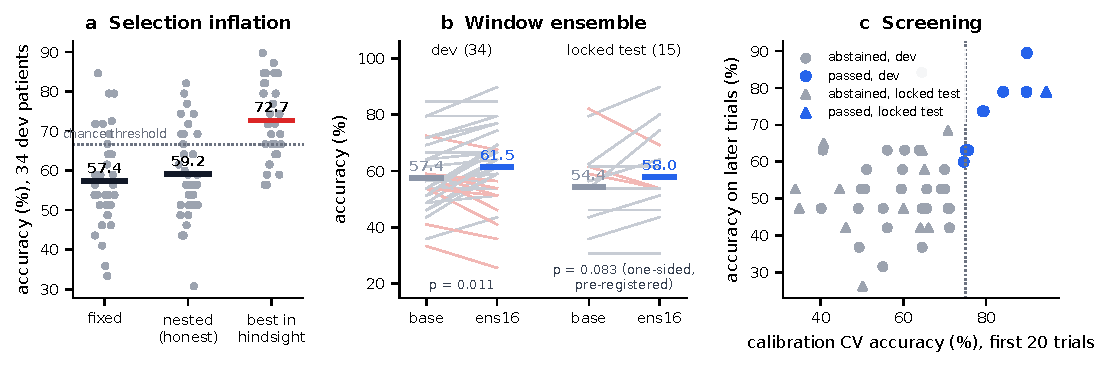
\includegraphics[width=\linewidth]{figures/fig5_beijing.pdf}
\caption{S1, left- versus right-hand imagery in acute stroke. \textbf{a}~Per-patient choice of window and band: fixed, chosen by nested cross-validation, and chosen in hindsight. The hindsight choice overstates accuracy by 13.5 points. \textbf{b}~Window ensemble versus base decoder for development and locked test patients; red lines mark patients harmed. \textbf{c}~Calibration accuracy on the first 20 trials (leave-one-pair-out) against accuracy on the later trials; patients passed by the gate in blue.}
\label{fig:beijing}
\end{figure}

\subsection{Few-trial calibration of affected-hand imagery versus rest (S3)}
\label{sec:s3}

Task~B is far easier: the own decoder reached 81.7\pct{} with five calibration pairs and 84.7\pct{} with ten (Figure~\ref{fig:strategies}).
\begin{itemize}
  \item \textbf{Deep transfer.} Every fine-tuned variant trailed the own decoder at both calibration sizes, by 4.5--12.2 points: healthy pretraining 76.6\pct{} and 76.3\pct{}, adding a LesionSim copy 76.3\pct{} and 76.5\pct{}, adding a generic-augmentation copy 74.5\pct{} and 72.5\pct{}, adding the other patients 77.2\pct{} and 76.3\pct{}. The deep models barely profited from twice as much calibration data.
  \item \textbf{Frozen foundation model.} The CBraMod probe trailed by 14--24 points (58.2--68.2\pct{}).
  \item \textbf{Riemannian pooling.} Pooling healthy donors into the re-centred Riemannian decoder did not help (78.9\pct{} and 84.3\pct{}), nor did LesionSim donors in population mode (79.7\pct{} and 84.2\pct{}) or patient-matched mode (78.6\pct{} and 83.5\pct{}).
\end{itemize}

Pooling the other development patients' recordings was the only strategy that improved on the own decoder. With five calibration pairs it reached 84.0\pct{}; median gain +1.4 points, $p = 0.004$, Holm-corrected $p = 0.018$; 11 of 16 patients helped and none harmed by 2 points or more. With ten pairs it reached 86.1\pct{} (+0.8 points, $p = 0.16$). The pre-registered test on the eight locked patients confirmed the five-pair result: 77.1\pct{} to 81.4\pct{}, one-sided $p = 0.035$, with 7 patients helped, 1 harmed, and all 8 above chance afterwards (Figure~\ref{fig:pooling}). Pooled decoding with five calibration pairs (81.4\pct{}) matched the own decoder with ten (79.5\pct{}), halving the calibration needed.

\begin{figure}[t]
\centering
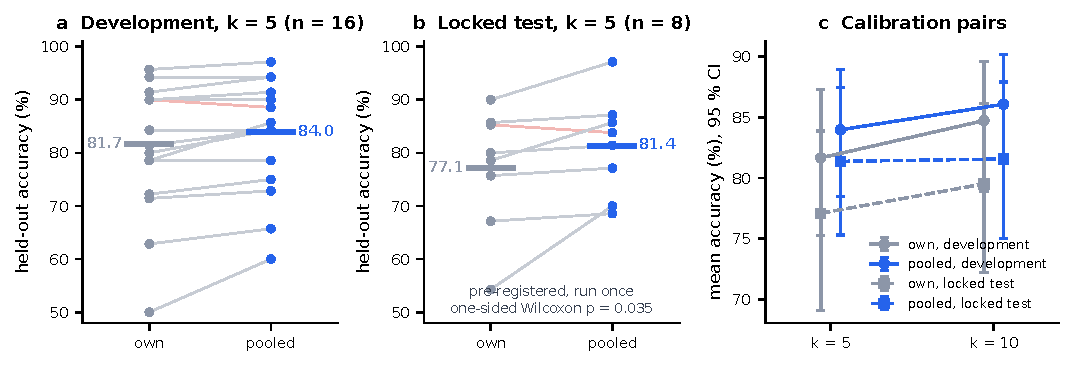
\includegraphics[width=\linewidth]{figures/fig1_pooling.pdf}
\caption{Pooling other patients' data into the re-centred Riemannian decoder (S3, Task~B). \textbf{a}~Development patients and \textbf{b}~locked test patients with five calibration pairs: each line is a patient, red when harmed; bars and numbers give means. \textbf{c}~Mean accuracy and bootstrap 95\pct{} confidence intervals with five and ten calibration pairs.}
\label{fig:pooling}
\end{figure}

\begin{figure}[t]
\centering
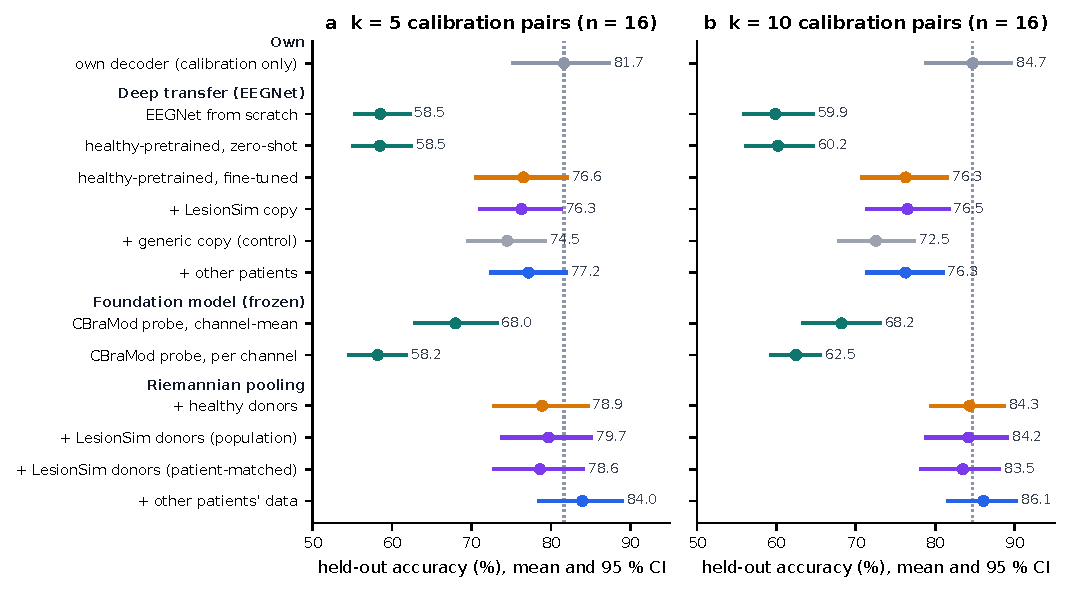
\includegraphics[width=\linewidth]{figures/fig2_transfer_strategies.pdf}
\caption{Sources of borrowed data for few-trial calibration (S3 development patients, Task~B), with \textbf{a}~five and \textbf{b}~ten calibration pairs. Points are means over 16 patients, lines bootstrap 95\pct{} confidence intervals; the dotted line marks the own decoder. Healthy data and LesionSim in every form, and the frozen foundation model, stay at or below the own decoder; only real patients' data improves on it.}
\label{fig:strategies}
\end{figure}

\subsection{LesionSim does not turn healthy donors into useful ones}
\label{sec:lesionsim}

Real patients were better donors than healthy participants by 5.1 points (84.0\pct{} vs 78.9\pct{} with five pairs). If LesionSim captured what distinguishes stroke data, its output should fall between the two. It did not.
\begin{itemize}
  \item All 27 learned settings scored between 78.5\pct{} and 80.0\pct{} (Figure~\ref{fig:lesionsim}).
  \item Chosen honestly across patients, the best setting gave 78.8\pct{}, no better than unmodified healthy donors (median $-0.7$ points, $p = 0.80$). It closed none of the gap; even the best setting in hindsight closed only 21\pct{} of it.
  \item The honestly chosen setting differed in every fold.
  \item In patient-matched mode, the estimated attenuation and shift mostly sat at their bounds: $\alpha = 1$ and $\beta = 1$ in the median. The chronic patients' ipsilesional mu desynchronisation was usually not weaker than the healthy participants' ($-13\pct{}$ ipsilateral and $-9\pct{}$ contralateral on average), contrary to the premise of operator O1.
\end{itemize}

\begin{figure}[t]
\centering
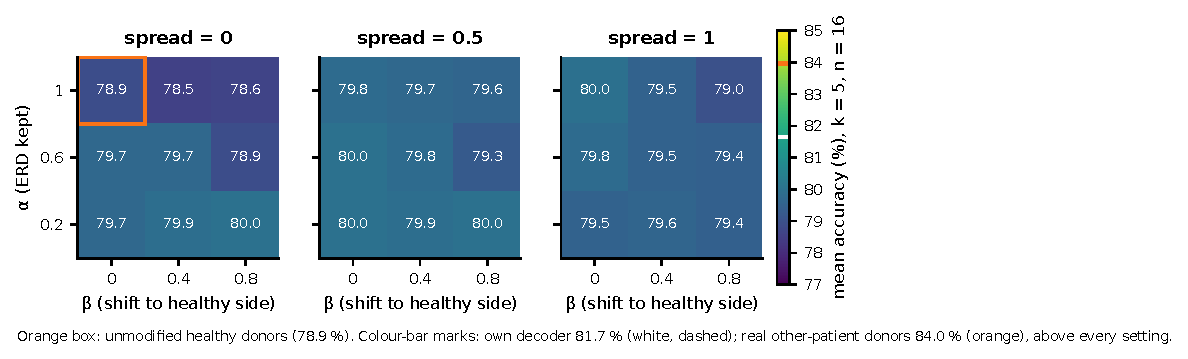
\includegraphics[width=0.86\linewidth]{figures/fig3_lesionsim_settings.pdf}
\caption{LesionSim with learned settings (S3 development patients, five calibration pairs). Each cell is the mean accuracy of the pooled decoder with healthy donors transformed by one setting of attenuation $\alpha$, contralesional shift $\beta$ and trial-to-trial spread. All settings stay far below real-patient donors.}
\label{fig:lesionsim}
\end{figure}

\subsection{SafeTransfer protects against harmful transfer}
\label{sec:gate}

When the transferred decoder was the LesionSim-pretrained EEGNet, always transferring harmed 9 of 16 development patients with five calibration pairs and 11 of 16 with ten. The gate harmed 2 and 1 (exact McNemar tests, $p = 0.008$ and $p = 0.001$; Figure~\ref{fig:gate}). It also raised mean accuracy over always transferring, by 4.2 points with five pairs (95\pct{} CI 0.0 to 8.6, $p = 0.033$) and by 8.1 points with ten (1.7 to 13.3, $p = 0.001$). The gate mostly kept the patient's own decoder. It did not beat always using the own decoder (80.6\pct{} vs 81.7\pct{} and 84.4\pct{} vs 84.7\pct{}). Its value is safety: when it is not known whether a transferred model helps a given patient, the gate decides from calibration data alone. With five pairs it abstained for 4 patients, and the remaining 12 reached 83.5\pct{}.

\begin{figure}[t]
\centering
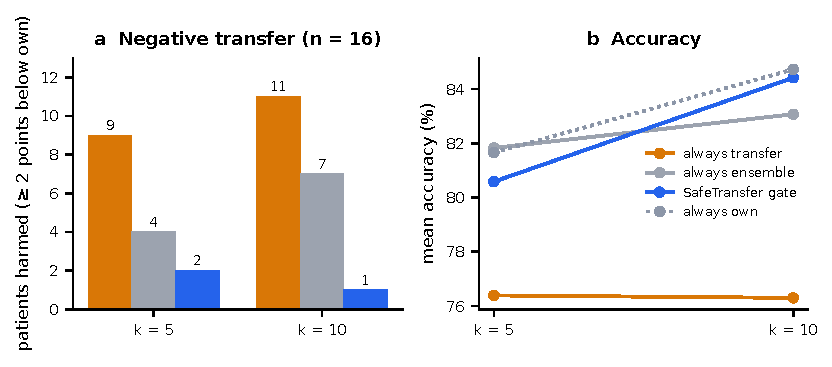
\includegraphics[width=0.78\linewidth]{figures/fig4_safetransfer.pdf}
\caption{SafeTransfer gate (S3 development patients). \textbf{a}~Patients harmed (at least 2 points below their own decoder) when always transferring, always averaging, or gating. \textbf{b}~Mean accuracy.}
\label{fig:gate}
\end{figure}

\subsection{Why other patients make better donors: neurophysiology}
\label{sec:neuro}

\paragraph{Stroke desynchronisation is stronger, wider and shifted, not weaker.} Relative to rest, the 24 chronic patients desynchronised more than the 109 healthy participants almost everywhere (Figure~\ref{fig:neuro}a).
\begin{itemize}
  \item In the mu band, patients reached $-17\pct{}$ to $-25\pct{}$ against $-6\pct{}$ to $-17\pct{}$ for healthy participants. The difference was significant at 11 of 14 channels (Holm-corrected Mann--Whitney tests). The exceptions were C3, Cz and CP3, where the healthy focus lies.
  \item In the beta band, the difference was significant at all 14 channels.
  \item Laterality reversed. Healthy desynchronisation was stronger over the hemisphere contralateral to the imagined hand. Patients' was stronger over the contralesional hemisphere: laterality index $+0.11$ versus $-0.10$ in mu and $+0.13$ versus $-0.17$ in beta, both $p < 0.001$.
\end{itemize}
The shift agrees with the contralesional recruitment reported in more impaired patients \citep{mansour2022}, and is what operator O2 imitates. The stronger ipsilesional desynchronisation contradicts the premise of operator O1. Recording system and paradigm also differ between the cohorts and may contribute to the overall difference in magnitude.

\paragraph{Patients' decision directions agree with each other.} In the re-centred tangent space, each patient's imagery-versus-rest direction was closer to the pooled direction of the other patients than to that of the healthy donors (median cosine 0.87 versus 0.78; Wilcoxon $p = 0.0002$; closer for 22 of 24 patients; Figure~\ref{fig:neuro}b). The within-patient split-half reliability, 0.92, is the ceiling: the other patients' direction comes close to what a second half of the patient's own data would give. This is the mechanism behind the pooling result. Re-centring removes each patient's average covariance, and what transfers is the direction. Other patients supply a direction almost as good as more of the patient's own data; healthy donors supply a biased one, and LesionSim did not correct the bias.

\paragraph{Decodability is stable across the study period.} The own decoder's accuracy did not change significantly between the three S3 time points (Figure~\ref{fig:neuro}c): 87.8\pct{} before ($n = 24$), 85.8\pct{} after ($n = 24$), and 85.6\pct{} at follow-up ($n = 19$). The post-minus-pre change was $-2.0$ points ($p = 0.18$) and follow-up minus pre $-2.1$ points (Holm-adjusted $p = 0.11$). Mu desynchronisation over C3 and C4 was also unchanged ($p = 0.46$ and $0.44$). A decoder calibrated in one session therefore faces a stable target in this cohort, and the pooled donor set does not need to be stratified by time point.

\begin{figure}[t]
\centering
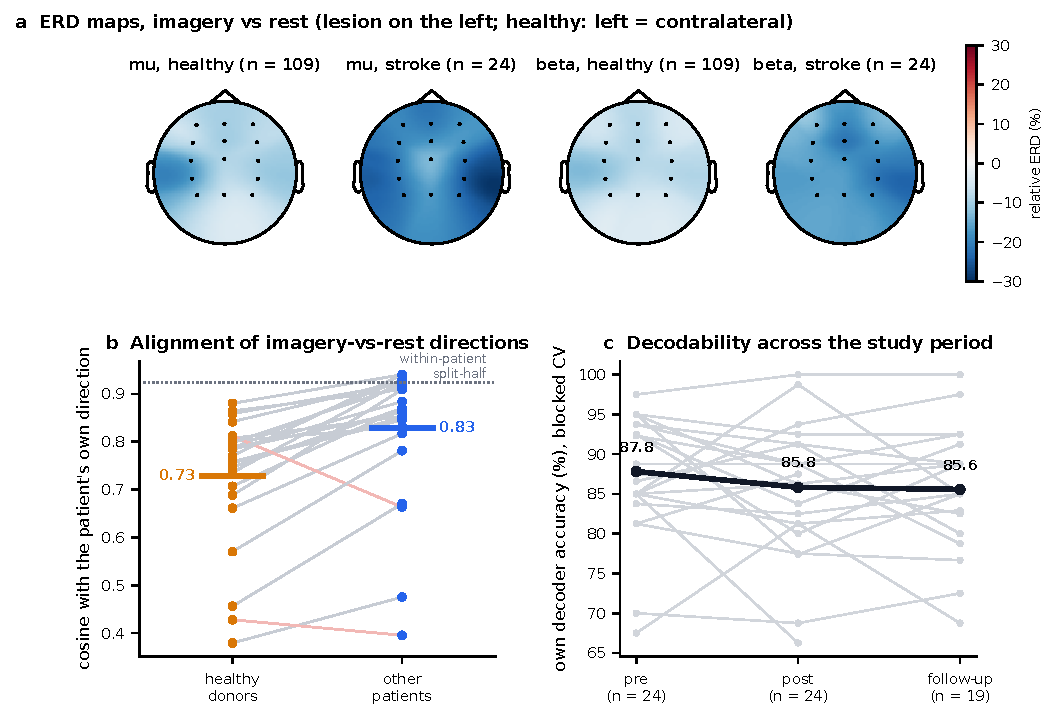
\includegraphics[width=\linewidth]{figures/fig6_neuro.pdf}
\caption{Neurophysiology of S3 (all 24 patients, descriptive; fixed methods). \textbf{a}~Relative desynchronisation during affected-hand imagery versus rest, averaged over participants, with the lesion on the left after harmonisation (for healthy participants, left is contralateral to the imagined right hand). \textbf{b}~Cosine between each patient's imagery-versus-rest direction and the pooled direction of healthy donors or of the other patients; the dotted line is the median within-patient split-half reliability. \textbf{c}~Own-decoder accuracy (blocked cross-validation) at the three time points.}
\label{fig:neuro}
\end{figure}


\subsection{Real-time operation}
\label{sec:online}

Streaming each S3 locked test patient's raw recording through the online pipeline reproduced the offline evaluation. With five calibration pairs, the own decoder averaged 77.1\pct{} online and offline, and the pooled decoder 82.5\pct{} online against 81.4\pct{} offline; per-patient differences came only from the causal filter. Processing took a median of 12.6\,ms per epoch in this streaming check. Over real Lab Streaming Layer streams, with the machine under full load, it took 21--23\,ms (maximum 54\,ms), and the final accuracies were identical to the streaming check. A decision is therefore available about 4\,s after each cue, at the end of the imagery window.

\section{Discussion}

Across two stroke cohorts and four ways of borrowing data, only one source helped a new patient with few calibration trials: other stroke patients. Pooling their recordings into a re-centred Riemannian decoder lifted accuracy with five rest--imagery pairs on never-seen patients, reaching what the patient's own decoder needed ten pairs for. Healthy recordings did not help in any form: as pretraining for a deep network, as donors for the Riemannian decoder, transformed by a physiology-based simulator in six variants, or distilled into a foundation model.

Why do real patients help when healthy participants do not? Re-centring removes each domain's average covariance, so what remains to transfer is the direction that separates imagery from rest. Healthy and stroke brains, recorded with different equipment and paradigms, differ in that direction more than stroke patients differ from each other (Section~\ref{sec:neuro}). LesionSim edits a few envelope statistics of healthy data, such as lesioned-side attenuation, contralesional shift and trial-to-trial variability. Even with learned settings this moved the healthy donors less than a quarter of the way toward real patients, and the patients it was meant to imitate did not show the assumed weaker lesioned-side desynchronisation. The practical conclusion is to pool real patient data across hospitals rather than synthesise it, and to share stroke recordings in harmonised form.

The results also bound what can be expected from left- versus right-hand imagery early after stroke with a portable 29-channel system and 40 trials. Most patients did not reach chance-adjusted significance with any decoder, and pretraining on the other patients did not change that. Calibration data identified who could, while clinical scores could not. A short screening session could therefore decide whether imagery-based feedback is worth offering, and the gate's abstention is the honest output for the rest.

Several evaluation pitfalls produced effects as large as the method differences studied here: hindsight selection (+13.5 points), transductive re-centring (+5 points) and a numerical failure of Euclidean alignment that manufactured negative transfer. Locked test sets, chronological calibration and pre-registered single-shot confirmation kept them out of the conclusions.

\paragraph{Limitations.}
\begin{itemize}
  \item The locked test sets are small (8 and 15 patients). The S3 confirmation rests on a one-sided test at $p = 0.035$, and the S1 locked set was used for two pre-registered hypotheses.
  \item All analyses are offline. The real-time system replays recordings rather than closing the loop with patients, and no clinical outcome was measured.
  \item Device and site are confounded with health status: healthy donors were recorded on a different system and paradigm from either stroke cohort. Part of the healthy-donor gap may therefore be technical rather than neurological. Same-device healthy controls (HEFMI-ICH) carried too little imagery signal to separate the two.
  \item LesionSim covers one family of envelope operators. A learned generative translation from healthy to stroke EEG was not attempted.
  \item A third left/right stroke cohort \citep{mathi2025} requires an access password that had not arrived at the time of writing.
\end{itemize}

\section{Conclusion}

For motor-imagery BCIs after stroke, data from other stroke patients shortens calibration, while healthy data, simulated stroke data and frozen foundation-model features do not. A re-centred Riemannian decoder pooled across patients halved the calibration needed on never-seen patients, and a calibration-only gate prevented harmful transfer. Building such systems will depend on shared, harmonised patient data rather than on simulating patients from healthy brains.

\section*{Data and code availability}
All datasets are public \citep{liu2024,wang2026,schalk2004,goldberger2000}. The code that rebuilds the harmonised benchmark, every experiment script, the per-patient result tables, the real-time implementation and the pre-registration log with its commit history are available at \url{https://github.com/prayag-1771/HemiShift}.


\bibliographystyle{unsrtnat}
\bibliography{refs}

\end{document}
